\section{Ziele}

\subsection{Visualisieren}
% successful
% unsuccessful

% Past Authoring:
% It is difficult to know who you are, where you should go, or how you should
% get there, unless you know where you came from. The Past Authoring Program
% has therefore been designed to help you write a structured autobiography. The
% program will help you:
% - Divide your life into seven different time periods or epochs.
% - Identify the most significant events that occurred during each epoch.
% - Describe how each of those experiences has shaped who you are today.



\begin{frame}[c]{Aufgabe: Gutes Visualisieren}
    Stell dir vor, welche:
    \begin{itemize}[<+(1)->]
        \item Art von Person du sein möchtest
        \item Fähigkeiten (Skills) du erlangt haben möchtest
        \item Beziehungen zu dir selbst, Freunden und Familie, Anderen, du haben möchtest
        \item Freizeitaktivitäten du genießen möchtest
    \end{itemize}
    \pause
    In den nächsten 6 Monaten / 3 Jahren / 5 Jahren?
    % Future Authoring:
    % specifically describe the type of person they wanted to be, the skills they wanted to attain, and the relationships they wanted to have, among other things
    % You will be asked to consider the people you admire, things you could do better, your educational and career goals, what habits you would like to improve, your family life, your social network, and your leisure activities.
    % timeframes: 6mo/2y/5y

    % source of positive emotion going forward

    % second part: detailed writing out how to do this
\end{frame}


\begin{frame}[c]{Aufgabe: Schlechtes Visualisieren}
    % the ways you are radically insufficient and your faults
    % how _you_ would degenerate
    % what is something you don't want to happen in 6mo/2y/5y
    Was passiert, wenn du:
    \begin{itemize}[<+(1)->]
        \item Deinen schlechten Gewohnheiten nachgibst
        \item Nicht auf deine Gesundheit achtest
        \item Dich von deinen Freunden entfernst
        \item Deine Ziele (wieder) nicht erreichst
    \end{itemize}
    \pause
    In den nächsten 6 Monaten / 3 Jahren / 5 Jahren?

\end{frame}



% \begin{frame}[c]{Was man erwarten kann}
%     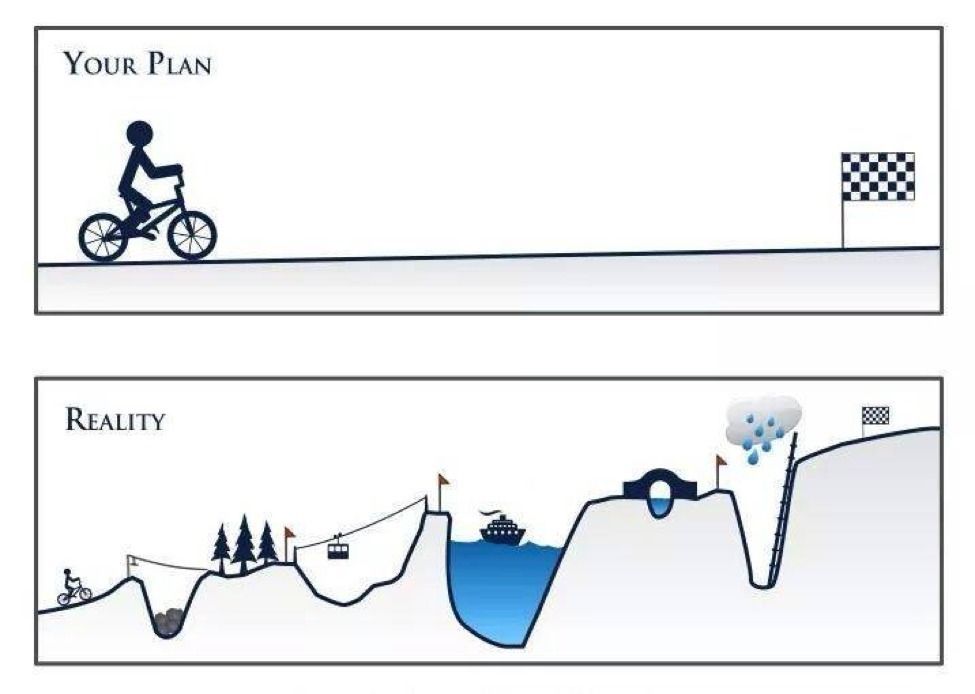
\includegraphics[height=0.8\textheight]{plan-reality} \\
%     Bild von \cite{plan-reality-pic-2}
% \end{frame}


\subsection{Finden}


\begin{frame}[c]{Aufgabe: Ziele aufschreiben}
    Regeln:
    \begin{itemize}[<+(1)->]
        \item Alles aufschreiben. Sortiert wird später
        \item Egal ob momentan Erreichbar oder nicht
        \item Langsam, Punkt für Punkt durchgehen
        \item Sei Ehrlich!
        \item Träume!
    \end{itemize}
\end{frame}



\begin{frame}[c]{Ziele Trigger List}
    \footnotesize
    % \begin{multicols}{2}
    \begin{itemize}
        % \item What would excite you, if you had the chance of doing?
        \item Worauf würdest du dich richtig freuen, wenn du die Möglichkeit dazu hättest?
        % \item What would make you fulfilled, if you had done it?
        \item Was würde dich erfüllen, wenn du es getan hättest?
        % \item What do you want to strive for? (e.g. World Peace, Revolutionizing Education, …)
        \item Wonach strebst du? (z.B. Weltfrieden, Kinder in Afrika retten, ...)
        % \item What would you do if there was no way to fail?
        \item Was würdest du tun, wenn du garantiert Erfolg hättest?
        % \item What do you want to have? (This can be material wants, achievements, …)
        \item Was möchtest du haben? (z.B. Materielles, Achievements, ...)
        % \item What do you want to be? (A great cook, fluent in French, …)
        \item Was wärst du gerne? (z.B. guter Koch, jemand Bewundernswertes, ...)
        % \item What would you do with 100 million in the bank?
        \item Was würdest du mit 100 Millionen auf dem Konto tun?
        % \item Which places would you want to go to?
        \item Was für Orte willst du besuchen?
        % \item What do you want to do before you die?
        \item Was würde auf deiner Bucket-List stehen?
        % \item What did you always want to learn, but never had the time for?
        \item Was wolltest du schon immer lernen?
        \item Was ist etwas, wofür du nie Zeit hattest?
    \end{itemize}
    % \end{multicols}
\end{frame}


\addtocounter{framenumber}{1}
\begin{frame}[standout]
    Machen (30min)
\end{frame}


\subsection{Reduzieren}

\addtocounter{framenumber}{1}
\begin{frame}[standout]
    \LARGE
    Achtung: Falls du die momentane Liste behalten willst, lohnt es sich, jetzt
    ein Foto oder eine Kopie davon anzulegen, da wir die Ziel-Liste im
    folgenden intensiv bearbeiten werden.
\end{frame}

\begin{frame}[c]{Vorbereitung}
    \Large
    Wandle alle Ziele, in denen du etwas {\em sein} möchtest, in ein Ziel um,
    in dem du etwas {\em tun} möchtest. \newline \newline \pause
    \textbf{Beispiel:} "guter Koch {\em sein}" $\rightarrow$ "so gut Kochen zu
    können, dass mir zugetraut wird, bei einer größeren Veranstaltung zu Kochen"
\end{frame}

\begin{frame}[c]{Aufgabe: Bedürfnisse finden}
    \normalsize
    Häufig sind Ziele nur Ersatz, um ein Bedürfnis zu füllen.
    \begin{itemize}[<+(1)->]
        \item Frage dich für jedes aufgeführte Ziel, \textbf{warum} du es tun möchtest
        \item Füge jedes neu gefundene \textbf{warum} zu deinen Zielen hinzu
        \item Wenn du das Ziel auch dann noch erreichen willst, wenn du das
            \textbf{warum} bereits auf einem anderen Weg erreicht hast, füge
            den Grund als weiteres 'warum' hinzu
        % \item Frage dich, ob du das Ziel immernoch erreichen wollen würdest,
        %     wenn du das \textbf{warum} auf einem anderen Weg erreichen
        %     könntest. Falls ja, füge das als weiteres 'warum' hinzu
        \item Entferne Ziele, dessen 'warum' bereits durch spannendere Ziele abgedeckt ist
    \end{itemize}
\end{frame}


\begin{frame}[c]{Aufgabe: Priorisieren}
    Manche Ziele sind spannender, und manche wichtiger als andere. Für jedes
    Ziel, frage dich:
    \begin{itemize}[<+(1)->]
        \item Ist es wirklich notwendig, das zu tun?
        \item Wie wichtig ist es mir, das zu erreichen?
        \item Wäre ich Zufrieden, wenn ich alles {\em außer} diesem Ziel schaffe?
    \end{itemize} \pause
    Versuche, 3-7 wirklich wichtige Ziele auszuwählen
\end{frame}



% \begin{frame}[c]{Theme}
%     Themes should be:
%     - Broad
%     - Directional
%     - Resonant <- most important
% \end{frame}
